% ----------------------------------
% Cap Análisis
% ----------------------------------
%	Incluye
%		Casos de uso
%
\documentclass[a4paper,oneside,11pt]{book}

\usepackage[spanish,activeacute]{babel}
\usepackage[utf8]{inputenc}
%\usepackage[T1]{fontenc}
\usepackage{tabulary}
\usepackage{graphicx}
\usepackage{color}
\usepackage{colortbl}
\usepackage{float}

\oddsidemargin=0.2cm
\headsep=1cm
\textheight=21cm
\textwidth=16cm

\setcounter{secnumdepth}{3}

\definecolor{gris}{gray}{0.80}
\definecolor{gris2}{gray}{0.90}
\definecolor{negro}{gray}{0}

% Personalizamos la separación entre párrafos...
\parskip=6pt

% Personalizamos el identado en la primera línea del nuevo párrafo...
\parindent=10pt

\begin{document}
	
\chapter{Diseño} % (fold)
\label{cha:diseno}


	\section{Diagramas de secuencia} % (fold)
	\label{sec:diagramas_de_secuencia}
	
		Cómo fue explicado en capítulos anteriores, los diagramas de interacción son diagramas que describen cómo grupos de objetos colaboran para conseguir algún fin. Estos diagramas muestran objetos, así como los mensajes que se pasan entre ellos dentro del caso de uso, es decir, capturan el comportamiento de los casos de uso.
		
		Hay dos tipos de diagrama de interacción, ambos basados en la misma información, pero cada uno enfatizando un aspecto particular: \textbf{Diagramas de Secuencia} y Diagramas de Colaboración.
	
		\medskip
		
		\fcolorbox{negro}{gris}{\parbox{15cm}{Un \textit{diagrama de Secuencia} muestra una interacción ordenada según la secuencia temporal de eventos. En particular, muestra los objetos participantes en la interacción y los mensajes que intercambian ordenados según su secuencia en el tiempo. Es decir, muestra la interacción de un conjunto de objetos en una aplicación a través del tiempo y se modela para cada caso de uso.}}
		
		\medskip
		
		En cuanto a la \textbf{representación}, el eje vertical representa el tiempo, y en el eje horizontal se colocan los objetos y actores participantes en la interacción, sin un orden prefijado. Cada objeto o actor tiene una línea vertical, y los mensajes se representan mediante flechas entre los distintos objetos. El tiempo fluye de arriba abajo. Se pueden colocar etiquetas (como restricciones de tiempo, descripciones de acciones, etc.) bien en el margen izquierdo o bien junto a las transiciones o activaciones a las que se refieren. 
		
		En este documento se detallan dos diagramas de secuencia hacen referencia a las \textit{Actividades Generales}. Son el de \textit{Buscar médico} y \textit{Ver información del médico.} Recordar que se utiliza el patrón de diseño modelo-vista-controlador.

		\newpage
		\subsection{Actividades generales} % (fold)
		\label{sub:actividades_generales}
		
			En primer lugar el diagrama de secuencia relacionado con el caso de uso \textit{Buscar médico}. En el interfaz principal de la aplicación, cuyo archivo para las vistas es \textit{index.html.erb}, nos aparece un cuadro de búsqueda en el que introducir los datos que deseamos, en este caso, el nombre y los apellidos del médico. La búsqueda se envía al controlador de dicha interfaz principal (\textit{welcome controller}), concretamente a la función \textit{search result}, y éste realiza una petición en la tabla \textit{doc}.
			
			Para realizar dicha petición, se unen previamente las columnas de \textit{name + apellido} de la tabla \textit{doc}, y luego se realiza la búsqueda. Por último, es este mismo controlador  (\textit{welcome controller}) el que se encarga de actualizar la vista del \textit{index.html.erb} mostrando los resultados obtenidos.
			
			\bigskip
			\bigskip
			
			\begin{figure}[H]
			  \centering
			    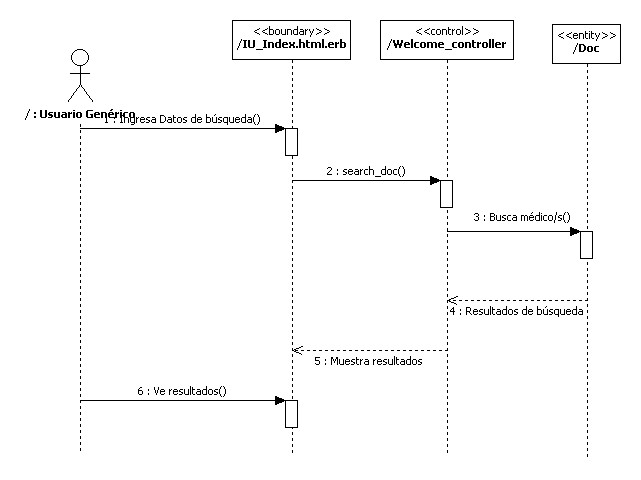
\includegraphics[width=16cm]{img/jpg/secuencia/01_BuscarMedico.jpg}
			  \caption{Buscar médico}
			  \label{fig:sec_general_buscarmedico}
			\end{figure}
			\newpage
			El segundo caso de uso llevado a estudio, y que posteriormente será implementado, es el de poder ver la información referente a un médico. Para ello, en la interfaz principal debemos previamente realizar una búsqueda. Los resultados obtenidos (médicos encontrados en función del nombre y apellidos introducidos) son \textit{links} en los que podemos hacer \textit{click} para acceder a ver la información.
			
			En este caso, el interfaz notificará al controlador \textit{doc controller} que el usuario ha seleccionado ver la información de un médico. Para ello se utiliza la acción \textit{show} del controlador. Se buscará el médico en la tabla \textit{doc} y a continuación se mostrará la vista relacionada con dicha acción, es decir, el \textit{show.html.erb} del médico seleccionado.
			\begin{figure}[H]
			  \centering
			    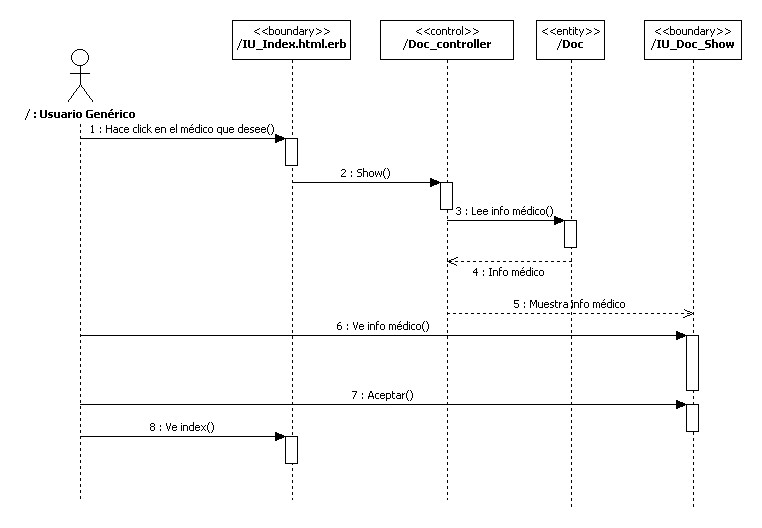
\includegraphics[width=16cm]{img/jpg/secuencia/02_VerInfoMedico.jpg}
			  \caption{Ver información del médico}
			  \label{fig:sec_general_verinfomedico}
			\end{figure}
			
		% subsection actividades_generales (end)
		
	% section diagramas_de_secuencia (end)

% chapter diseno (end)

\end{document}